\documentclass[14pt]{extarticle}
\usepackage[margin=1in]{geometry}
\usepackage{verbatim}
\usepackage{times}
\usepackage{graphicx}
\usepackage{float}
\begin{document}
\title{Big Data Assignment 2: Hadoop MapReduce Experimentation}
\author{Lee Boyd \\
        Corey Crosser \\
        Sean Soderman
        }
\date{\today}
\maketitle

\section{Representative Console Screenshot}
\begin{figure}[H]
\centering
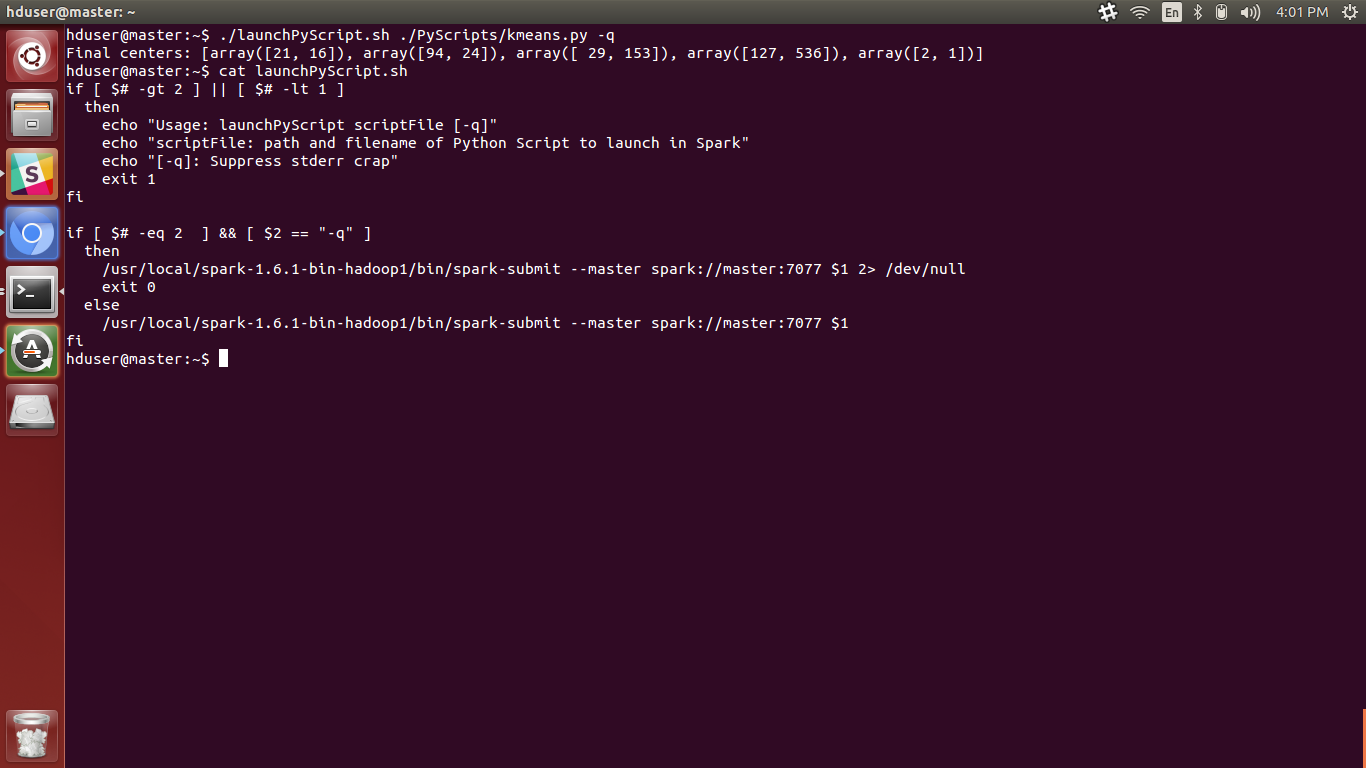
\includegraphics[width=5.2in]{conoutput.png}
%\caption{}
\end{figure}

\section{Web Interface Screenshot}
\begin{figure}[H]
\centering
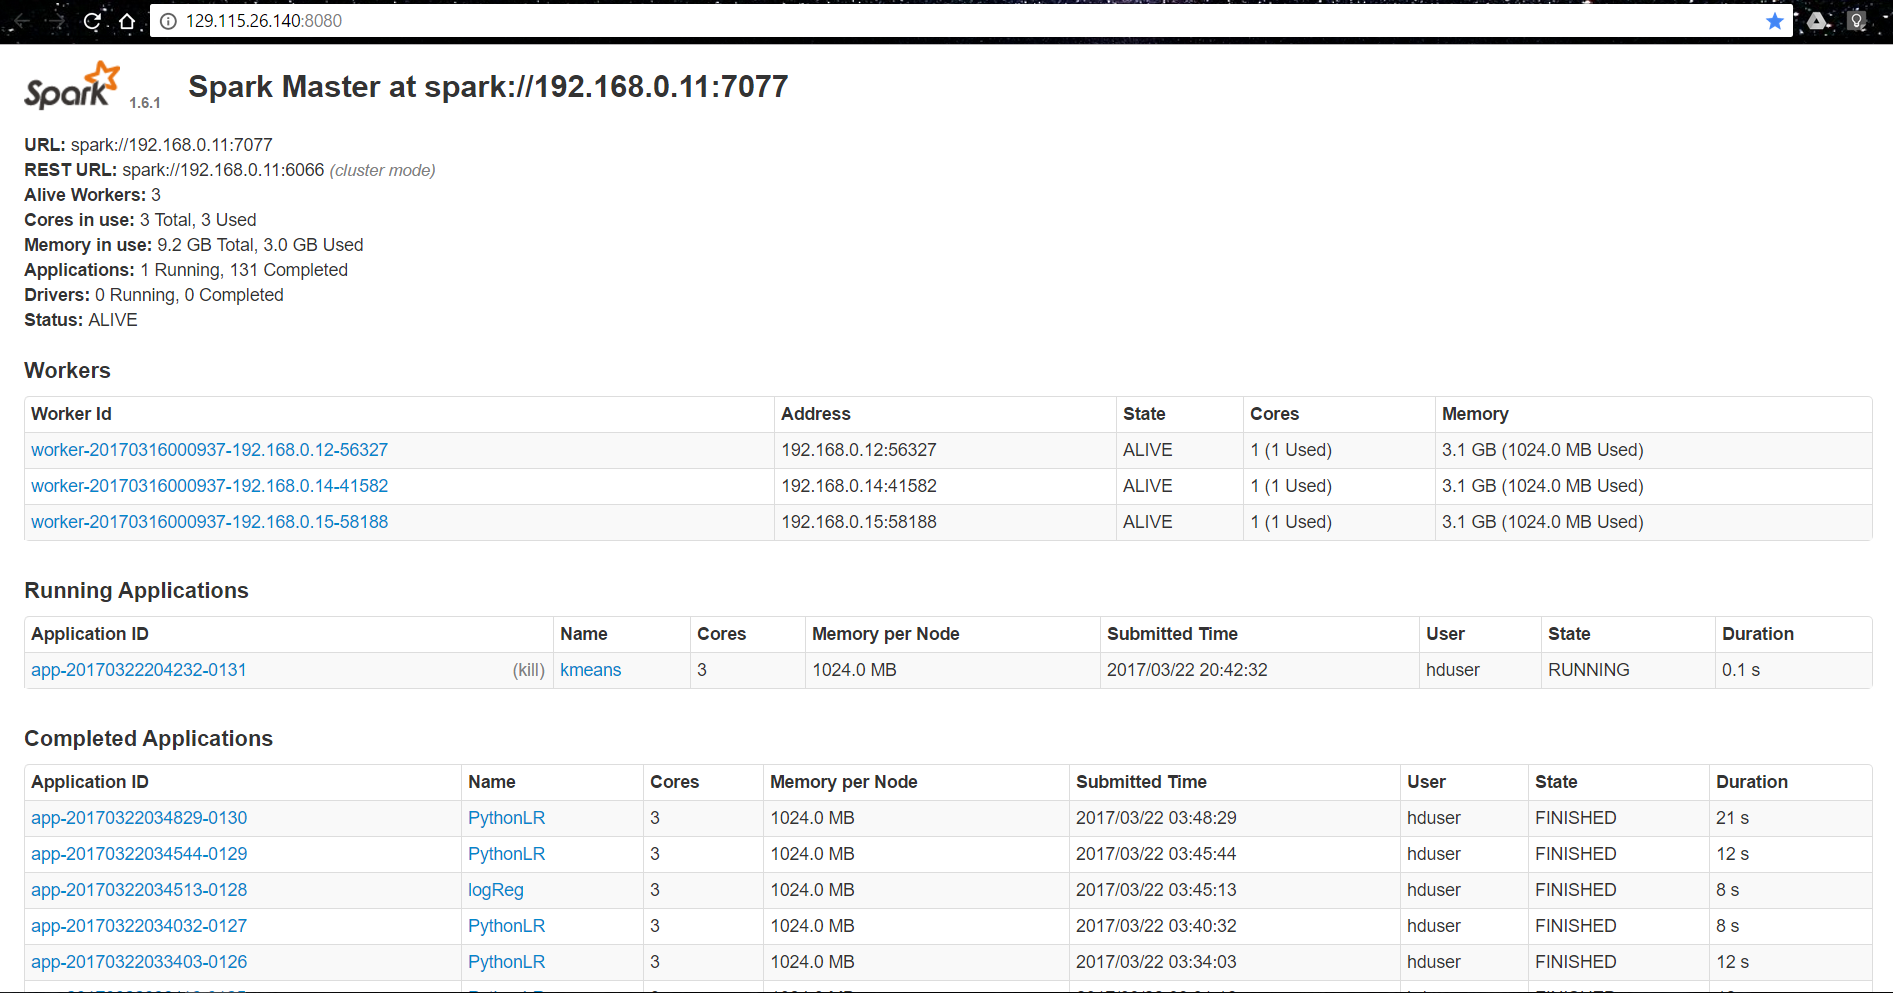
\includegraphics[width=5.2in]{SparkScreenShot.png}
%\caption{}
\end{figure}

\section{Work Division Description}
Corey set up the systems as well as developed an overall architecture for the k-means
algorithm in Spark.

Lee and Sean worked on implementing k-means.

%TODO: Need to write more stuff?


\end{document}
